\documentclass[12pt]{article}
\usepackage[T1, T2A]{fontenc}
\usepackage[utf8]{inputenc}
\usepackage[russian]{babel}
\usepackage{hyperref}
\usepackage{graphicx}
\graphicspath{ {../Images/} }

\author{Григорий Матюхин}
\date{\today}
\title{Лабораторная работа \textnumero7.\\Управление журналами событий}

\begin{document}
\maketitle
\newpage
\tableofcontents
\newpage
\section{Цель работы}
Получить навыки работы с журналами мониторинга различных событий в системе.

\section{Последовательность выполнения работы}

\subsection{Мониторинг журнала системных событий в реальном времени}
\begin{enumerate}
	\item Запустите три вкладки терминала и в каждом из них получите полномочия администратора:
	\item На второй вкладке терминала запустите мониторинг системных событий в реальном времени:
	\item В третьей вкладке терминала вернитесь к учётной записи своего пользователя и попробуйте получить полномочия администратора, но введите неправильный пароль. Обратите внимание, что во второй вкладке терминала с мониторингом событий или ничего не отобразится, или появится сообщение \texttt{FAILED SU (to root) username ...}. Отображаемые на экране сообщения также фиксируются в файле \texttt{/var/log/messages}.
	      \\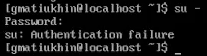
\includegraphics{1.png}
	      \\
\includegraphics{2.png}
	\item В третьей вкладке терминала из оболочки пользователя введите \texttt{logger hello}. Во второй вкладке терминала с мониторингом событий вы увидите сообщение, которое также будет зафиксировано в файле /var/log/messages.
	      \\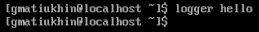
\includegraphics{3.png}
	      \\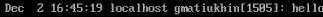
\includegraphics{4.png}
	\item Во второй вкладке терминала с мониторингом остановите трассировку файла сообщений мониторинга реального времени. Затем запустите мониторинг сообщений безопасности (последние 20 строк соответствующего файла логов). Вы увидите сообщения, которые ранее были зафиксированы во время ошибки авторизации при вводе команды \texttt{su}.
	      \\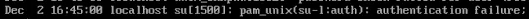
\includegraphics{5.png}
\end{enumerate}

\subsection{Изменение правил rsyslog.conf}
По умолчанию веб-служба не регистрирует свои сообщения через \texttt{rsyslog}, а пишет свой собственный журнал (в каталоге \texttt{/var/log/httpd}). Настройте регистрацию сообщений веб-службы через \texttt{syslog}, создав правило, регистрирующее отладочные сообщения в отдельном лог-файле. Для этого выполните следующие действия.
\begin{enumerate}
	\item В первой вкладке терминала установите Apache, если он не был ранее инсталлирован:
	\item После окончания процесса установки запустите веб-службу:
	      \\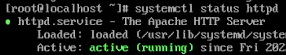
\includegraphics{6.png}
	\item Во второй вкладке терминала посмотрите журнал сообщений об ошибках вебслужбы:
	      \\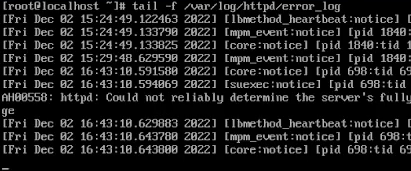
\includegraphics{7.png}
	\item В третьей вкладке терминала получите полномочия администратора и в файле конфигурации \texttt{/etc/httpd/conf/httpd.conf} в конце добавьте следующую строку: \texttt{ErrorLog syslog:local1}. Здесь \texttt{local0} — \texttt{local7} — это «настраиваемые» средства (объекты), которые \texttt{syslog} предоставляет пользователю для регистрации событий приложения в системном журнале:
	      \\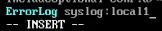
\includegraphics{8.png}
	\item В каталоге \texttt{/etc/rsyslog.d} создайте файл мониторинга событий веб-службы. Открыв его на редактирование, пропишите в нём \texttt{local1.* -/var/log/httpd-error.log}. Эта строка позволит отправлять все сообщения, получаемые для объекта \texttt{local1} (который теперь используется службой \texttt{httpd}), в файл \texttt{/var/log/httpderror.log}:
	      \\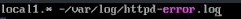
\includegraphics{9.png}
	\item Перейдите в первую вкладку терминала и перезагрузите конфигурацию \texttt{rsyslogd} и веб-службу. Все сообщения об ошибках веб-службы теперь будут записаны в файл \texttt{/var/log/httpd-error.log}, что можно наблюдать или в режиме реального времени, используя команду \texttt{tail} с соответствующими параметрами, или непосредственно просматривая указанный файл:
	      \\
\includegraphics{10.png}
	\item В третьей вкладке терминала создайте отдельный файл конфигурации для мониторинга отладочной информации. Открыв его на редактирование, пропишите в нём \texttt{*.debug /var/log/messages-debug}
	      \\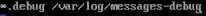
\includegraphics{11.png}
	\item В первой вкладке терминала снова перезапустите \texttt{rsyslogd}:
	\item Во второй вкладке терминала запустите мониторинг отладочной информации:
	\item В третьей вкладке терминала введите \texttt{logger -p daemon.debug "Daemon Debug Message"}:
	      \\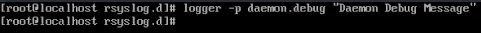
\includegraphics{12.png}
	\item В терминале с мониторингом посмотрите сообщение отладки:
	      \\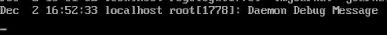
\includegraphics{13.png}
\end{enumerate}

\subsection{Использование journalctl}
\begin{enumerate}
	\item Во второй вкладке терминала посмотрите содержимое журнала с событиями с момента последнего запуска системы:
	      \\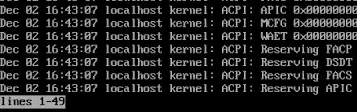
\includegraphics{14.png}
	\item Просмотр содержимого журнала без использования пейджера:
	      \\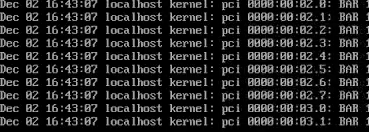
\includegraphics{15.png}
	\item Режим просмотра журнала в реальном времени:
	      \\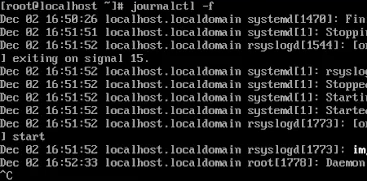
\includegraphics{16.png}
	\item Просмотрите события для \texttt{UID0}:
	      \\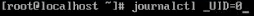
\includegraphics{17.png}
	\item Для отображения последних 20 строк журнала введите:
	      \\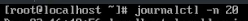
\includegraphics{18.png}
	\item Для просмотра только сообщений об ошибках введите:
	      \\
\includegraphics{19.png}
	\item Если вы хотите просмотреть сообщения журнала, записанные за определённый период времени, вы можете использовать параметры \texttt{--since} и \texttt{--until}. Обе опции принимают параметр времени в формате \texttt{YYYY-MM-DD hh:mm:ss}. Кроме того, вы можете использовать \texttt{yesterday}, \texttt{today} и \texttt{tomorrow} в качестве параметров. Например, для просмотра всех сообщений со вчерашнего дня введите:
	      \\
\includegraphics{20.png}
	\item Если вы хотите показать все сообщения с ошибкой приоритета, которые были зафиксированы со вчерашнего дня, то используйте:
	      \\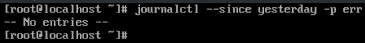
\includegraphics{21.png}
	\item Если вам нужна детальная информация, то используйте \texttt{journalctl -o verbose}:
	      \\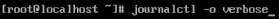
\includegraphics{22.png}
	\item Для просмотра дополнительной информации о модуле sshd введите \texttt{journalctl \_SYSTEMD\_UNIT=sshd.service}:
	      \\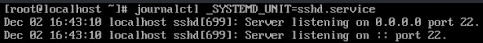
\includegraphics{23.png}
\end{enumerate}

\subsection{Постоянный журнал journald}
По умолчанию журнал journald хранит сообщения в оперативной памяти системы и записи доступны в каталоге \texttt{/run/log/journal} только до перезагрузки системы. Для того чтобы сделать журнал \texttt{journald} постоянным, выполните следующие действия:
\begin{enumerate}
	\item Запустите терминал и получите полномочия администратора:
	\item Создайте каталог для хранения записей журнала:
	\item \label{access} Скорректируйте права доступа для каталога \texttt{/var/log/journal}, чтобы \texttt{journald} смог записывать в него информацию:
	      \\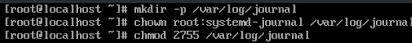
\includegraphics{24.png}
	\item Для принятия изменений необходимо или перезагрузить систему (перезапустить службу \texttt{systemd-journald} недостаточно), или использовать команду \texttt{killall -USR1 systemd-journald}:
	      \\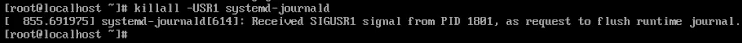
\includegraphics{25.png}
	\item Журнал systemd теперь постоянный. Если вы хотите видеть сообщения журнала с момента последней перезагрузки, используйте \texttt{journalctl -b}:
\end{enumerate}

\section{Контрольные вопросы}
\begin{enumerate}
	\item Какой файл используется для настройки \texttt{rsyslogd}? \\
	      Главный файл конфигурации \texttt{rsyslog} - \texttt{/etc/rsyslog.conf}. Он загружает модули, определяет глобальные директивы, содержит правила по обработке сообщений логов, а также включает пути ко всем файлам конфигурации в директории \texttt{/etc/rsyslog.d/} для различных приложений и служб.
	\item В каком файле журнала \texttt{rsyslogd} содержатся сообщения, связанные с аутентификацией? \\
	      \texttt{/var/log/secure}
	\item Если вы ничего не настроите, то сколько времени потребуется для ротации файлов журналов? \\
	      По умолчанию \texttt{logrotate} производит ротацию раз в день.
	\item Какую строку следует добавить в конфигурацию для записи всех сообщений с приоритетом \texttt{info} в файл \texttt{/var/log/messages.info}? \\
	      \texttt{*.info /var/log/messages.info}
	\item Какая команда позволяет вам видеть сообщения журнала в режиме реального времени? \\
	      \texttt{tail -f /var/log/messages}
	\item Какая команда позволяет вам видеть все сообщения журнала, которые были написаны для \texttt{PID 1} между 9:00 и 15:00? \\
	      \texttt{journalctl \_PID=1 --since 09:30 --until 15:00}
	\item Какая команда позволяет вам видеть сообщения \texttt{journald} после последней перезагрузки системы? \\
	      \texttt{journalctl -b}
	\item Какая процедура позволяет сделать журнал \texttt{journald} постоянным? \\
	      \begin{enumerate}
		      \item Создайте каталог для хранения записей журнала с необходимыми правами доступа (см. \ref{access})
		      \item Перезагрузить систему или выполнит комманду \texttt{killall -USR1 systemd-journald}
	      \end{enumerate}
\end{enumerate}

\section{Вывод}
В ходе выполнения данной работы я получил навыки работы с журналами мониторинга различных событий в системе.

\end{document}
